\documentclass[runningheads]{llncs}

\usepackage{graphicx}
\usepackage{booktabs}
\usepackage{amsmath}
\usepackage{amssymb}
\usepackage{tikz}
\usetikzlibrary{arrows.meta,positioning,fit,calc}
\usepackage{xcolor}
\usepackage{array}
\usepackage{multirow}
\usepackage{enumitem}
\setlist{itemsep=1pt, topsep=3pt, parsep=0pt, partopsep=0pt}

\begin{document}

\title{Bounded-Authority Agent Specialization for Adaptive Technical Interview Systems: Coordination, Safeguards, and Empirical Trade-offs}
\titlerunning{Bounded-Authority Agent Specialization for Adaptive Interview Systems}

\author{Anonymous Author(s)}
\authorrunning{Anonymous et al.}
\institute{Anonymous Institution}

\maketitle

\begin{abstract}
Interview-practice systems may be described as multi-agent even when one controller invokes components procedurally. We ask whether two bounded-authority agents, a Strategy Agent and a Coaching Agent, with threshold-gated arbitration over a frozen Proximal Policy Optimization (PPO) policy, change decisions in an adaptive technical-interview system, and whether any change arises from specialization or from coordination. Using 160 deterministic replay sessions (8 replay clusters $\times$ 20 question-order permutations; no live LLM), the agent layer altered difficulty trajectories relative to the frozen single-controller baseline, with fewer level changes ($15.12 \rightarrow 12.45$) and lower PPO agreement ($0.626 \rightarrow 0.400$); a cluster bootstrap over the 8 structural clusters gave a level-change difference of $-2.67$ [$-4.50$, $-0.24$], and leave-one-cluster-out analysis showed this magnitude was sensitive to individual clusters. Under matched open-loop replay, a specialized two-agent implementation and a unified controller produced identical decisions on all 1,280 turns ($P(\mathrm{agree}) = 1.0$), and the coordination layer added $+1.04$\,ms median per-turn latency. Fault injection showed containment of tested adversarial proposals when arbitration was active (0/40 sessions with guardrail bypass) versus 38/40 without it; a separate lexical grounding probe accepted unsupported paraphrased credit in all 57 of 57 applicable cases, showing the validator enforces an evidence contract rather than semantic correctness. Results are limited to deterministic replay with fixed candidate responses; no claim is made that specialization is behaviorally superior to a unified controller, and no human-learning claim is made.

\keywords{multi-agent coordination \and agent specialization \and decision-making \and trajectory dynamics \and interview practice \and arbitration}
\end{abstract}

\section{Introduction}

Adaptive technical-interview systems make a sequence of decisions rather than evaluating each response independently: evidence from one turn influences later question difficulty, follow-up behavior, and feedback, so local choices accumulate into a trajectory. A centralized policy is a straightforward way to maintain this control loop (evaluated responses become a state representation, a policy produces an action, and an authoritative system commits the decision), and it simplifies state consistency and decision ownership. It also couples responsibilities that may operate at different temporal scales, since longitudinal progression and localized feedback need not require the same information or reasoning. When they share a single decision path, it is difficult to tell whether behavior changes arise from the underlying policy, from the interaction between distinct responsibilities, or from the mechanism that reconciles competing recommendations.

Decomposing decision-making across specialized components provides one way to expose these relationships. Separating responsibilities can make state ownership explicit and allow different components to maintain information relevant to their respective roles. However, decomposition alone does not establish a behavioral advantage. Once multiple components can produce recommendations, their communication, proposal constraints, and arbitration mechanism become part of the decision process. An observed change in behavior may therefore result from coordination rather than specialization itself. Conversely, a specialized architecture may alter the organization and isolation of state without changing the decisions ultimately produced under equivalent conditions. Distinguishing these effects is necessary for understanding what a multi-agent architecture contributes to an adaptive decision system.

This paper studies that distinction in an automated technical-interview preparation system with an authoritative session-state hub and a single-policy reinforcement-learning controller for adaptive difficulty. The system evaluates technical responses and uses accumulated session information to determine subsequent actions. We extend this established decision pipeline with a bounded-authority coordination layer in which specialized components maintain separate private state and communicate through constrained proposals, while final state commitment remains centralized. This arrangement makes the path from observation to proposal, arbitration, and commitment explicit without transferring authoritative state mutation to the participating agents.

The resulting architecture provides a controlled setting for separating several properties that are often treated collectively as evidence of a multi-agent design. Coordination concerns the effect of introducing auxiliary proposals into an existing decision loop. Specialization concerns the division of responsibility and state across distinct components rather than a unified controller. Arbitration determines how competing recommendations are admitted and resolved against the underlying policy, while authority mechanisms determine which components are permitted to influence committed state and how invalid or unsafe proposals are contained. Treating these properties separately allows the behavioral consequences of coordination to be distinguished from the architectural consequences of specialization. What existing agent-oriented and safe-reinforcement-learning literature does not establish is how such a bounded-authority layer actually behaves once it is inserted into an already-operating adaptive controller -- specifically, which of its claimed properties survive deterministic replay, targeted fault injection, mechanism-level ablation, and a direct specialized-versus-unified comparison, rather than being assumed from the architecture diagram alone.

The study therefore asks (RQ1) whether adding bounded multi-agent coordination changes the dynamics of adaptive interview decisions and follow-up probing relative to the original single-controller system; (RQ2) whether dividing responsibility across specialized stateful components changes decisions when the surrounding observations, rules, and arbitration conditions are held constant; (RQ3) which arbitration mechanisms determine whether auxiliary proposals influence the resulting trajectory; and (RQ4) whether bounded proposal authority and downstream safeguards preserve authoritative state and system invariants in the presence of component failures and adversarial proposals. These questions are examined through deterministic replay and controlled architectural comparisons designed to isolate the relevant variables rather than treating the number of agents as the experimental variable of interest.

This study makes three contributions. First, a \emph{behavioral-testing methodology} for an added coordination layer that combines deterministic REPLAY, FAULT-INJECTED, and SYNTHETIC evidence under a single replay harness, rather than evaluating the layer only on held-out task outcomes. Second, \emph{property-specific testing of coordination safeguards} -- confidence-gated arbitration, schema and authority validation, concept grounding, and a per-agent circuit breaker -- through controlled ablation (Experiment XA), a registered threshold sweep (Experiment XC), and targeted fault injection (Experiment XB), so that a given safeguard's necessity is tied to a specific tested property rather than asserted globally. Third, an \emph{empirical characterization of specialization and its limits}, including negative findings: two registered predictions (A9, A10) were contradicted by the data, and a matched specialized-versus-unified comparison found no decision difference under the tested conditions. We do not claim that multi-agent specialization is behaviorally superior to a unified controller, that the observed trajectory change reflects improved candidate outcomes, or that the tested safeguards establish general fault tolerance; Sect.~8 states these boundaries in full.

The remainder of the paper moves from architecture to evidence: Sections~2--4 position the work and specify the architecture, authority topology, and arbitration; Section~5 describes the controlled comparisons; Sections~6--7 present and interpret the findings; and Sections~8--9 state the limitations and conclusions.

\section{Related Work}

Research on multi-agent systems has established several ways of distributing complex decision processes across interacting components. Classical agent-oriented work emphasizes autonomy, reactivity, pro-activeness, and social interaction as fundamental properties of agents \cite{wooldridge1995}. More recent LLM-based systems operationalize these ideas through structured collaboration. AutoGen, for example, uses conversational interaction as a mechanism for coordinating multiple agents \cite{autogen2023}, while MetaGPT organizes agents around specialized roles and standardized workflows \cite{metagpt2024}. These approaches show that dividing responsibility can structure complex tasks, but behavior depends also on how information and intermediate decisions move between agents.

This distinction becomes important when architectural organization is evaluated empirically. Studies comparing different agent configurations have reported task-dependent rather than universally superior arrangements \cite{kim2026artifact,kim2026outgrow}. In addition, evaluations centered on final task artifacts can obscure the internal mechanism responsible for an observed difference: a change in outcome may arise from role specialization, from the information exchanged between agents, or from the coordination procedure that determines how their outputs are combined. Recent analyses of multi-agent systems have similarly identified failures involving specification, inter-agent alignment, and verification \cite{cemri2025}, indicating that the organization of interaction is itself an important part of the system being evaluated. The question is therefore not simply whether several agents can collectively solve a task, but whether the architectural separation of responsibilities changes the decisions produced when the surrounding information and decision conditions are held constant.

We treat adaptive interviewing as a sequential decision problem in which accumulated session evidence determines subsequent interactions. Reinforcement learning is one framework for mapping an observed state to actions over a sequence of decisions; our system uses PPO \cite{schulman2017} as implemented in Stable-Baselines3 \cite{raffin2021}. In a technical interview, however, the information relevant to longitudinal assessment progression need not be identical to the information used for feedback, hints, or follow-up behavior. A centralized controller can therefore couple responsibilities that operate on different aspects of an evolving interaction. When the controller acts on a compact representation of a longer session, an individual decision also affects the state encountered at later turns, making the resulting trajectory an important object of analysis rather than merely a sequence of independent actions.

Separating assessment progression from coaching-related responsibilities may change the organization and ownership of state without changing the final decisions, whereas introducing additional decision sources can alter the trajectory through the mechanism used to admit and reconcile their proposals. The two effects are easy to conflate when decomposition and coordination are introduced simultaneously, so a controlled evaluation needs to distinguish them.

Safety-oriented reinforcement learning provides the complementary principle that adaptive decisions need not possess unrestricted authority. Shielding and supervisory approaches place external constraints around learned policies so that unsafe actions can be rejected, overridden, or restricted before they reach the environment \cite{alshiekh2018,garcia2015}. This separation between policy generation and authoritative enforcement becomes particularly relevant when additional stateful components are introduced. A component may maintain information relevant to its role and recommend an action without being permitted to modify the authoritative state directly. Such a distinction allows proposal generation, validation, arbitration, and final commitment to be treated as separate responsibilities rather than allowing every participating component to act as a state owner. The principle of least privilege \cite{saltzer1975} gives this separation a general systems-security justification independent of the reinforcement-learning setting.

Containment of component failures is a related but distinct concern from containment of unsafe policy actions. Fault-injection practice in production software systems deliberately introduces failures to observe whether surrounding safeguards contain them rather than assuming containment from design intent alone \cite{basiri2016}, and interface-level contracts that specify what a component may and may not do, and what happens when a call violates that contract, are an established way to make such containment checkable \cite{meyer1992}. The present study applies both ideas to an agent boundary: typed proposal contracts play the role of Meyer's interface contracts, and the fault-injection campaign (Experiment XB, Sect.~5) plays the role of a deliberately injected failure against which containment is checked, rather than assumed.

Once several components can contribute recommendations, the system must determine which information each component owns, what authority accompanies a proposal, how proposals are reconciled with the underlying policy, and which constraints remain authoritative when they conflict. These questions require the internal decision path to be observable if their individual effects are to be separated experimentally.

The literature consequently provides the principal building blocks for distributed responsibility, sequential adaptation, and supervisory constraint enforcement, while leaving open an important empirical distinction between coordination and specialization. Distributed state and role separation may change the architecture without changing matched decisions, whereas coordination and arbitration may directly affect the trajectory through which decisions are produced. Authority boundaries add a further dimension by determining whether those distributed components remain subordinate to a single authoritative state owner. The present study uses this distinction as the basis for its architecture: specialized components maintain bounded private state and communicate constrained proposals, while authoritative commitment remains centralized. The architectural structure required to make those distinctions explicit is described next.

\section{System Architecture and Authority Topology}

\textbf{Reference Monolithic Workflow.} A browser client sends a spoken answer to a backend, which transcribes it and calls an \texttt{InterviewOrchestrator} (the hub; Fig.~1). The hub owns one session-state dictionary and one lock and runs a fixed per-turn pipeline: (1) a learned \emph{evaluator} (sentence-embedding similarity $S_1$, a concept index $S_2$ and a fine-tuned cross-encoder $R$; $0.15S_1 + 0.35S_2^{\mathrm{eff}} + 0.50R$ with a cap when a mandatory concept is missed) returns a score and concept evidence; (2) a strict hand-off contract treats a non-finite or out-of-range score as an evaluator failure and fails closed; (3) feedback is produced by a template or an optional local LLM; (4) the hub commits the turn; (5) a baseline schedule and then a frozen PPO policy \cite{raffin2021,schulman2017} propose an easier/same/harder action, followed by a rule layer of six guardrails; (6) a threshold rule decides whether a follow-up question is injected (at most two in a row). Before this work only the PPO policy was a reactive learned decision-maker; the LLM never chose an action. All of this is unchanged when the multi-agent flag is off, and a test shows that with the flag on but no agent contributing the trajectory is identical (Sect.~6).

\begin{table}[t]
\caption{Authority matrix, generated from the enforcing code (\texttt{agents/multiagent/authority.py}). Neither agent has state-write authority; the hub commits alone.}
\label{tab:authority}
\centering
\resizebox{\textwidth}{!}{%
\begin{tabular}{@{}p{1.4cm}p{3.1cm}p{3.1cm}p{4.6cm}p{3.0cm}@{}}
\toprule
\textbf{Agent} & \textbf{May propose} & \textbf{Private state} & \textbf{Cannot} & \textbf{On invalid output} \\
\midrule
Strategy & difficulty\_action (Easier/Same/Harder); probe request (concept, kind); strategy mode &
weakness ledger (per-concept miss counts, probe history, trend) &
write or overwrite any score; set a difficulty level directly; terminate the session; edit history; override hard constraints or guardrail overrides; call another agent &
invalid / stale / low-confidence / timed-out proposal is dropped; PPO proposal stands \\
\addlinespace
Coaching & feedback depth; hint / example flags; concepts to emphasise; remediation tag; tone &
coaching history (hints/examples given, repeated misconceptions) &
alter evaluator results or scores; cite concepts absent from the evaluator evidence; request difficulty changes; request follow-ups; terminate the session &
invalid plan is dropped; the existing template feedback is used unchanged \\
\bottomrule
\end{tabular}%
}
\end{table}

\textbf{Specialized Agent Roles and Private State.} Table~1 lists what each agent may propose and may not do. Applying the principle of least privilege \cite{saltzer1975}, neither agent possesses state-write privileges. Both agents implement a single method \texttt{propose(observation, peer)}, receive an immutable, validated \texttt{TurnObservation} (score, evidence lists, difficulty, score history, progress, follow-up counters; counters carry the value the hub will commit), and return a typed proposal. They are rule- and ledger-based, not LLM-driven; they are the smallest design that has private persistent state, pro-active proposals and a communication channel, which are the properties of weak agency \cite{wooldridge1995} that the existing roles lacked. We make no claim of autonomy beyond that.

\textbf{Strategy Agent.} Objective: maintain configured difficulty adaptation while tracking persistent weaknesses within the follow-up budget. Private state: per concept, the distinct turns in which the evaluator listed it as missing or incorrect, which concepts were later covered, probes already requested, and an exponential moving average (EMA) of scores. Rules, first match wins: \emph{recover} (current score $<0.35$ and mean of the last two $<0.5$, or a weakness that survived its probes while the score stays $<0.5$) $\rightarrow$ Easier; \emph{remediate} (a concept missed on $\geq 2$ distinct turns and unresolved) $\rightarrow$ Same plus a probe request for that concept; \emph{stretch} (score $\geq 0.8$, average $\geq 0.7$, last three $\geq 0.6$, no open weakness) $\rightarrow$ Harder; otherwise \emph{steady}. Non-steady proposals use confidence $\min(0.95, 0.5+0.1n)$ for $n$ cited evidence items (a documented heuristic rather than a calibrated probability), while steady proposals are assigned 0.45 (below the arbitration threshold $\tau=0.6$, so the PPO action stands unless the ledger supports a change).

\textbf{Coaching Agent.} Objective: choose how to coach after an evaluated answer. Private state: concept miss counts and the hints and examples already given. Decisions: up to two concepts to emphasize (incorrect claims first, then repeatedly missed, then evaluator order); a hint if concepts are missing, the score is $<0.6$ and fewer than two hints were given for the lead concept; an example when the lead concept was missed before and no example was given yet; depth (\emph{detailed} if score $<0.4$ or a repeated miss, \emph{brief} if $\geq 0.85$ with nothing missing); tone; a remediation tag. A Strategy proposal delivered as a peer message modifies the plan (\emph{recover}: detailed and encouraging; \emph{stretch}: brief; \emph{remediate}: remediation tag on the probed concept). A deterministic renderer applies the plan to the existing feedback dictionary: it adds presentation fields and may prepend a priority tip to, or truncate, the existing improvement and communication-tip lists, and it raises if any protected evaluator field (score, grade, concept and claim lists, transcript, decision source) would change.

\textbf{Communication and State Ownership.} Every observation, proposal and decision is a typed object (pydantic, unknown fields rejected, NaN and out-of-range values rejected). The coordinator records each call as an envelope with session, turn, sender, recipient, state version and provenance, and every accept/reject/modify outcome as a decision record with a reason code -- this per-call envelope and per-decision reason code are the observability substrate the ablation (Sect.~6) and fault-injection (Sect.~5) analyses read from. Optimistic concurrency uses a state version that counts committed turns: a proposal whose version, turn or session differs from the observation, or from the hub's current version, is stale and dropped; a second answer from the same agent for the same version is a duplicate and dropped. The hub builds observations, commits state, increments the version, and persists agent memory in its session snapshot so that a recovered session resumes with the agents' ledgers.

\begin{figure}[t]
\centering
\resizebox{!}{6.4cm}{%
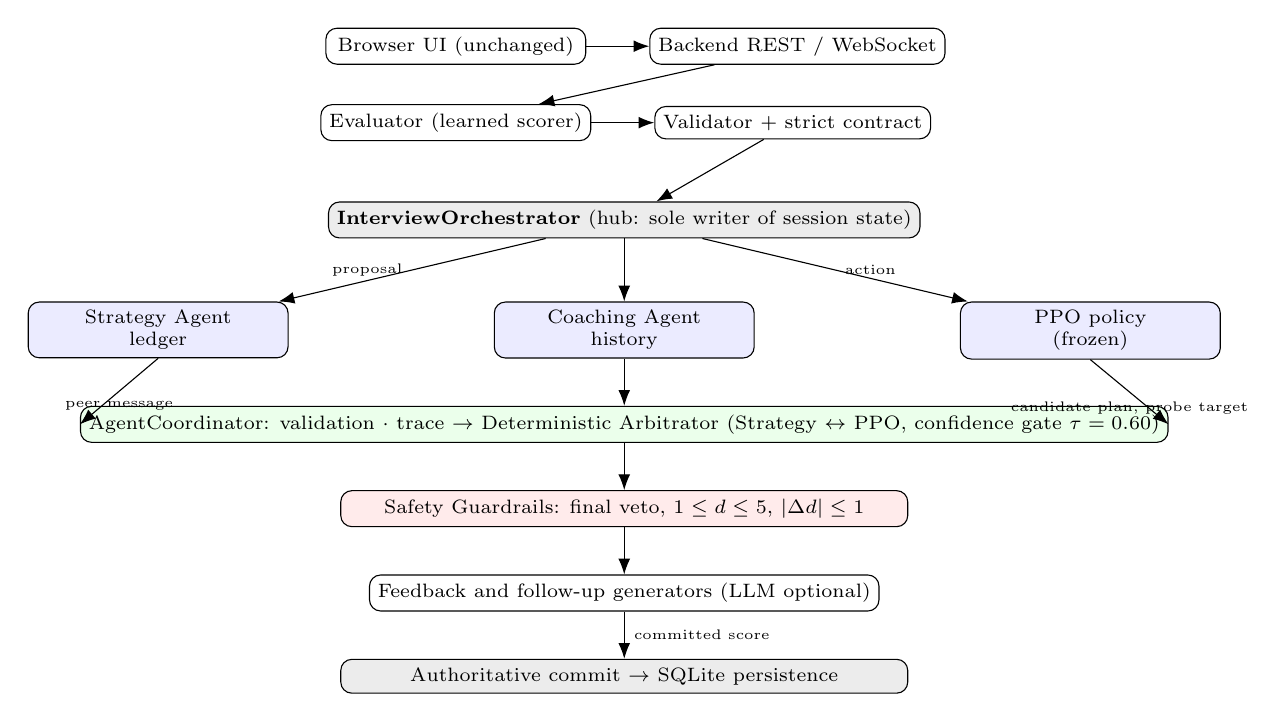
\begin{tikzpicture}[
  node distance=5mm and 8mm,
  box/.style={draw, rounded corners, align=center, font=\scriptsize, inner sep=3pt},
  hub/.style={box, fill=gray!15, minimum width=7.2cm},
  agent/.style={box, fill=blue!8, minimum width=3.3cm},
  guard/.style={box, fill=red!8, minimum width=7.2cm},
  io/.style={box, minimum width=3.3cm},
  arr/.style={-{Latex[length=2mm]}, font=\tiny}
]
\node[io] (ui) {Browser UI (unchanged)};
\node[io, right=of ui] (backend) {Backend REST / WebSocket};
\node[io, below=of ui] (evaluator) {Evaluator (learned scorer)};
\node[io, right=of evaluator] (validator) {Validator + strict contract};
\node[hub, below=10mm of $(evaluator)!0.5!(validator)$] (hub) {\textbf{InterviewOrchestrator} (hub: sole writer of session state)};
\node[agent, below left=8mm and 5mm of hub] (strategy) {Strategy Agent\\ledger};
\node[agent, below=8mm of hub] (coaching) {Coaching Agent\\history};
\node[agent, below right=8mm and 5mm of hub] (ppo) {PPO policy\\(frozen)};
\node[box, fill=green!8, below=6mm of coaching, minimum width=7.2cm] (coord) {AgentCoordinator: validation $\cdot$ trace $\rightarrow$ Deterministic Arbitrator (Strategy $\leftrightarrow$ PPO, confidence gate $\tau=0.60$)};
\node[guard, below=6mm of coord] (guardrails) {Safety Guardrails: final veto, $1 \le d \le 5$, $|\Delta d| \le 1$};
\node[io, below=6mm of guardrails] (feedback) {Feedback and follow-up generators (LLM optional)};
\node[hub, below=6mm of feedback] (commit) {Authoritative commit $\rightarrow$ SQLite persistence};

\draw[arr] (ui) -- (backend);
\draw[arr] (backend) -- (evaluator);
\draw[arr] (evaluator) -- (validator);
\draw[arr] (validator) -- (hub);
\draw[arr] (hub) -- (strategy) node[midway, left, font=\tiny] {proposal};
\draw[arr] (hub) -- (coaching);
\draw[arr] (hub) -- (ppo) node[midway, right, font=\tiny] {action};
\draw[arr] (strategy.south) -- (coord.west) node[midway, below, font=\tiny] {peer message};
\draw[arr] (coaching) -- (coord);
\draw[arr] (ppo.south) -- (coord.east) node[midway, below, font=\tiny] {candidate plan, probe target};
\draw[arr] (coord) -- (guardrails);
\draw[arr] (guardrails) -- (feedback);
\draw[arr] (feedback) -- (commit) node[midway, right, font=\tiny] {committed score};
\end{tikzpicture}%
}
\caption{System architecture and authority topology of the bounded multi-agent configuration. The \texttt{InterviewOrchestrator} retains sole authority over committed session state. Strategy and Coaching maintain separate private ledgers and contribute proposal-only outputs. Strategy may transmit a unidirectional operational mode to Coaching, while both components submit typed proposals to the coordinator. The PPO policy independently provides the baseline difficulty action. The coordinator routes eligible proposals to deterministic arbitration, after which downstream guardrails retain final veto authority before the hub commits the resulting state transition.}
\label{fig:architecture}
\end{figure}

\section{Orchestration, Arbitration and Validation}

Figure~2 shows one turn. \textbf{Difficulty precedence} (deterministic code, evaluated by ablation rather than assumed optimal): (1) hard constraints (infrastructure failure forces Same; levels stay in $[1,5]$); (2) the guardrail layer, applied last to whichever candidate was selected, wins whenever a rule fires (G3 and G6 hold or raise difficulty, so this layer does not act solely in a downward direction); (3) a validated Strategy proposal with confidence $c \geq \tau$ and cited evidence supersedes the PPO action, recorded as a \emph{conflict}; (4) the PPO action, or the labeled non-RL heuristic when PPO is unavailable. A proposal that cannot take effect at the bounds is recorded as \emph{modified}. \textbf{Probe precedence}: the hard cap of two consecutive follow-ups, then a Strategy probe whose concept appeared in the evaluator's evidence earlier in this session and whose confidence satisfies $c \geq \tau$ (it may add a probe the thresholds would not trigger, or retarget the default one), then the hub's original threshold rule. The retargeted concept is passed to the template follow-up generator; the LLM prompt is not changed.

\textbf{PPO integration.} PPO keeps its role and its 6-D state and 3-action definitions; the reference policy was trained once with a fixed configuration and seed (seed 123, 100,000 nominal training steps) and then frozen before the multi-agent evaluation; no hyperparameter search or result-based checkpoint selection was performed. That training run is itself SIMULATED evidence from prior work, distinct from the REPLAY, FAULT-INJECTED, and SYNTHETIC evidence classes this study produces for the coordination layer (Sect.~5); the present study treats the checkpoint as a frozen artifact and does not retrain or re-select it. Its action is one input to arbitration. The agents never see the PPO action before they propose, and the paper makes no claim that the agents improve PPO. Calling this multi-agent RL would be wrong: one policy is learned, and the agents are not trained.

\textbf{Guardrails.} The deployed hub uses an inline copy of the rule layer that differs from the module used by the training environment. A configuration key selects \texttt{legacy\_inline} (default; deployed behavior) or \texttt{canonical}, both are reported separately. On a synthetic grid (39,930 points, hesitation $hes = 1-conf$, with $conf$ the acoustic confidence) the two disagree on 4,728 points (11.8\%) in G2, G6 and the no-override case; this is a property of the grid, not a deployment frequency, and a regression test pins it.

\begin{figure}[t]
\centering
\resizebox{!}{4.6cm}{%
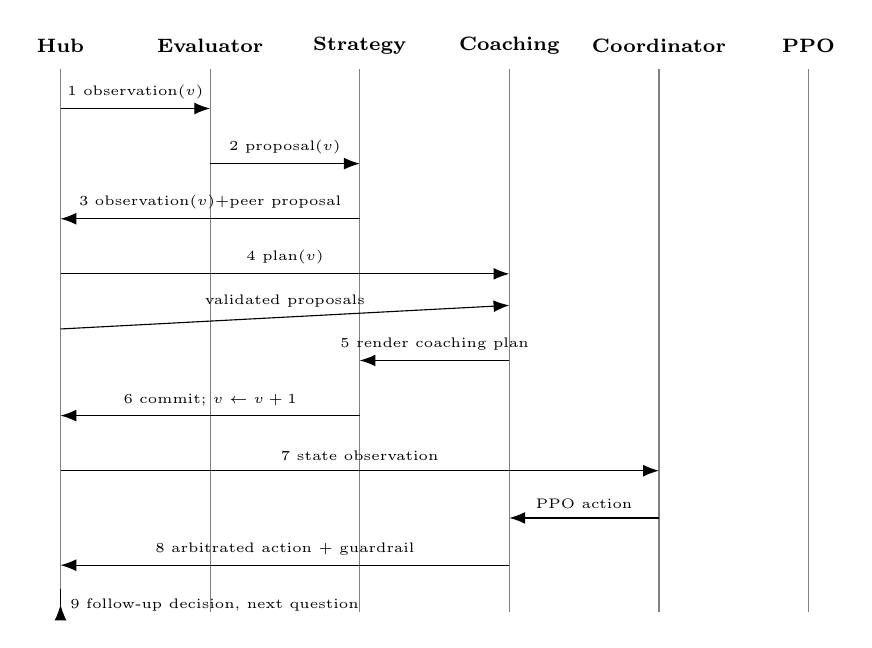
\begin{tikzpicture}[
  font=\scriptsize,
  line/.style={-{Latex[length=2mm]}},
  dashline/.style={-{Latex[length=2mm]}, dashed}
]
\def\lanes{Hub,Evaluator,Strategy,Coaching,Coordinator,PPO}
\foreach \name [count=\i] in \lanes {
  \node[font=\bfseries\scriptsize] (head\i) at (\i*1.9, 0) {\name};
  \draw[gray] (\i*1.9, -0.3) -- (\i*1.9, -7.2);
}
\draw[line] (1.9,-0.8) -- (3.8,-0.8) node[midway, above, font=\tiny]{1 observation($v$)};
\draw[line] (3.8,-1.5) -- (5.7,-1.5) node[midway, above, font=\tiny]{2 proposal($v$)};
\draw[line] (5.7,-2.2) -- (1.9,-2.2) node[midway, above, font=\tiny]{3 observation($v$)+peer proposal};
\draw[line] (1.9,-2.9) -- (7.6,-2.9) node[midway, above, font=\tiny]{4 plan($v$)};
\draw[line] (1.9,-3.6) -- (7.6,-3.3) node[midway, above, font=\tiny]{validated proposals};
\draw[line] (7.6,-4.0) -- (5.7,-4.0) node[midway, above, font=\tiny]{5 render coaching plan};
\draw[line] (5.7,-4.7) -- (1.9,-4.7) node[midway, above, font=\tiny]{6 commit; $v \leftarrow v+1$};
\draw[line] (1.9,-5.4) -- (9.5,-5.4) node[midway, above, font=\tiny]{7 state observation};
\draw[line] (9.5,-6.0) -- (7.6,-6.0) node[midway, above, font=\tiny]{PPO action};
\draw[line] (7.6,-6.6) -- (1.9,-6.6) node[midway, above, font=\tiny]{8 arbitrated action + guardrail};
\draw[line] (1.9,-7.1) -- (1.9,-7.1) node[right, font=\tiny]{9 follow-up decision, next question};
\end{tikzpicture}%
}
\caption{One interview turn as implemented (verbal path). Steps 1--4 happen before the hub commits; arbitration (8) follows the PPO suggestion. On the code-submission path only the Strategy proposal is collected.}
\label{fig:turn}
\end{figure}

\begin{figure}[t]
\centering
\resizebox{!}{4.8cm}{%
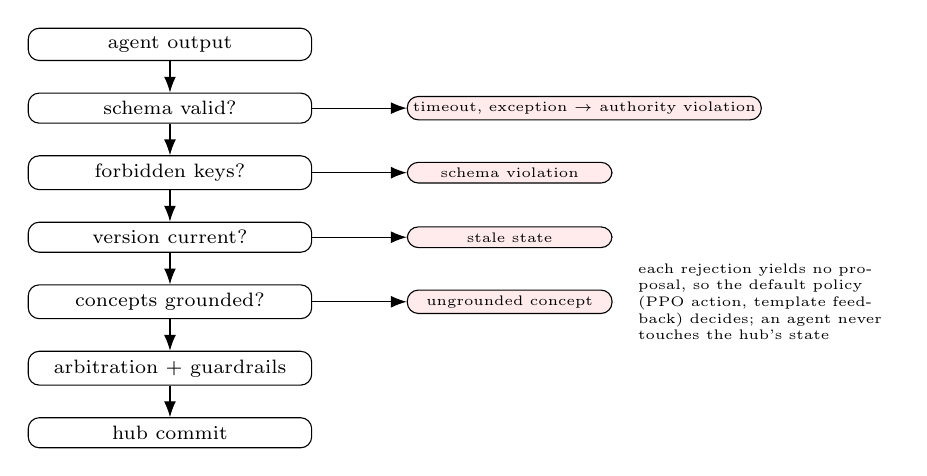
\begin{tikzpicture}[
  font=\scriptsize,
  node distance=4mm,
  box/.style={draw, rounded corners, align=center, inner sep=3pt, minimum width=3.6cm},
  rej/.style={draw, rounded corners, align=center, inner sep=2pt, fill=red!8, font=\tiny, minimum width=2.6cm},
  arr/.style={-{Latex[length=2mm]}}
]
\node[box] (c1) {agent output};
\node[box, below=of c1] (c2) {schema valid?};
\node[box, below=of c2] (c3) {forbidden keys?};
\node[box, below=of c3] (c4) {version current?};
\node[box, below=of c4] (c5) {concepts grounded?};
\node[box, below=of c5] (c6) {arbitration + guardrails};
\node[box, below=of c6] (c7) {hub commit};
\draw[arr] (c1) -- (c2); \draw[arr] (c2) -- (c3); \draw[arr] (c3) -- (c4);
\draw[arr] (c4) -- (c5); \draw[arr] (c5) -- (c6); \draw[arr] (c6) -- (c7);
\node[rej, right=12mm of c2] (r2) {timeout, exception $\rightarrow$ authority violation};
\node[rej, right=12mm of c3] (r3) {schema violation};
\node[rej, right=12mm of c4] (r4) {stale state};
\node[rej, right=12mm of c5] (r5) {ungrounded concept};
\draw[arr] (c2) -- (r2); \draw[arr] (c3) -- (r3); \draw[arr] (c4) -- (r4); \draw[arr] (c5) -- (r5);
\node[font=\tiny, right=2mm of r5, text width=3.2cm, align=left] {each rejection yields no proposal, so the default policy (PPO action, template feedback) decides; an agent never touches the hub's state};
\end{tikzpicture}%
}
\caption{Validation pipeline every proposal passes before arbitration. Each rejection yields no proposal; the default policy decides.}
\label{fig:validation}
\end{figure}

\textbf{Proposal Validation.} Before any proposal reaches arbitration, the coordinator executes four sequential checks (Fig.~3): (1) strict Pydantic schema validation (\texttt{extra=forbid}, NaN and out-of-range rejection); (2) recursive scanning against the 18 forbidden state keys; (3) optimistic concurrency verification matching the hub's current committed turn version; and (4) concept evidence grounding. If an agent raises an unhandled exception or exceeds the configured timeout (150\,ms), its proposal is dropped and the hub proceeds with the default policy.

\section{Experimental Methodology}

\textbf{Evaluation Environment and Replay Dataset.} To evaluate coordination and specialization without stochastic variance from live network calls, all experiments run via deterministic replay through the real orchestrator hub with \texttt{EVALUATOR\_MOCK\_MODE=1}. All experiments operate on a fixed set of 64 technical-interview replay instances across eight underlying replay clusters prepared for the proposed system, combining constructed (authored) answer payloads with team-generated/synthetic instances. Each replay cluster corresponds to the $k$-th recorded answer set across the eight interview questions ($k=1,\ldots,8$). In replay mode, the hub consumes these fixed evaluator inputs directly, driving the full state machine and coordinator. Evidence classes are labeled by experiment: REPLAY (XA, XC, and the open-loop split versus unified comparison), FAULT-INJECTED (XB, faults injected into the real agents during replay), and SYNTHETIC (the authored feedback probes of XD and the guardrail state-grid analysis). For follow-up probes, the replay reuses the recorded evaluator payload associated with the root concept rather than generating a new candidate response. Replay sessions combine the 8 underlying replay clusters with 20 question orders (order seeds 0--19; seed 0 is the original order), yielding $N=160$ sessions per experimental condition. These 160 sessions are \emph{not} independent; they reuse the identical 8 replay clusters. We therefore explicitly model the 8 underlying replay clusters as the independent structural units in the cluster-aware analyses. No live generative LLM is invoked during replay; the LLM gateway is stubbed as down and deterministic template renderers handle text output, so trajectory differences are evaluated under fixed stimuli without live-model stochasticity. Per-turn latency was timed in-process with a monotonic wall-clock timer around each orchestrator call, with the order of conditions within each replay cell shuffled to control drift. Runs used Python 3.11 with dependency versions outside the repository's pins; CPU, hardware, and operating-system details were not recorded, so latency is reported as a paired overhead between conditions rather than as absolute performance.

\textbf{Baseline and Ablation Matrix.} To address RQ1 (coordination dynamics), RQ3 (coordination mechanisms), and RQ4 (authority and safety boundaries), we evaluate the baseline platform alongside controlled ablation conditions (Experiment XA) across the identical 160 replay sessions:
\begin{itemize}
\item \textbf{Frozen Baseline (B0):} Single-controller workflow without agents, with PPO active and deployed inline guardrails.
\item \textbf{PPO-Disabled Baseline (B7):} Single-controller baseline with PPO unavailable, using deterministic rule fallback.
\item \textbf{Canonical-Guardrail Baseline (B0c):} Baseline evaluated with canonical \texttt{rl/guardrails.py} instead of inline rules.
\item \textbf{Full Multi-Agent System (M1):} Strategy and Coaching agents, peer messaging, and arbitration ($\tau=0.6$).
\item \textbf{Strategy Agent Ablated (M2):} Strategy disabled while Coaching and the coordination layer remain active.
\item \textbf{Coaching Agent Ablated (M3):} Coaching disabled while Strategy remains active, testing trajectory independence.
\item \textbf{Arbitration Ablated (M4):} Raw Strategy proposals admitted without confidence-threshold, evidence-grounding, or step-bound checks.
\item \textbf{Grounding Verification Ablated (M5):} Coaching plans accepted without concept-evidence grounding checks.
\item \textbf{Peer Communication Ablated (M6):} Strategy-to-Coaching peer messaging disabled, isolating message exchange.
\item \textbf{Authority Enforcement Ablated (M8):} Score authority verification bypassed before proposal admission.
\item \textbf{PPO-Disabled Multi-Agent (M7):} Full multi-agent system with PPO disabled, falling back to rule heuristic (paired with B7).
\item \textbf{Canonical-Guardrail Multi-Agent (M1c):} Full multi-agent system evaluated with canonical guardrails.
\end{itemize}

\textbf{Framework for Evaluating Agent Specialization (RQ2).} To evaluate whether decomposing technical coaching into specialized agents produces measurable behavioral divergence or operational trade-offs compared to a unified controller (RQ2), we formulate a controlled comparative framework contrasting: (1) \textbf{Specialized Architecture ($M_{\mathrm{split}}$}): The two-agent baseline (M1) partitioning responsibilities across Strategy and Coaching with separate state ledgers and explicit peer messaging; and (2) \textbf{Unified Architecture ($M_{\mathrm{unified}}$}): A monolithic agent (\texttt{UnifiedCoachAgent}) maintaining a joint session ledger and synthesizing difficulty actions, follow-up probes, and coaching plans in a single dispatch. To ensure an equivalent comparison, both configurations receive identical observation inputs, identical question sequences, identical heuristic decision thresholds, and identical arbitration rules. We evaluate four measured outcomes alongside one architectural property: (1) decision agreement rate ($P(\mathrm{Decision}_{\mathrm{unified}} = \mathrm{Decision}_{\mathrm{split}})$); (2) difficulty-action agreement and (3) follow-up probe agreement, both components of (1); (4) per-turn dispatch and serialization latency; and (5) architectural state encapsulation (schema separation and separate ledger boundaries).

\textbf{Threshold Decomposition (Experiment XC).} Because the unarbitrated condition (M4) simultaneously removes the confidence threshold, evidence verification, and one-step limits, it cannot isolate which mechanism prevents oscillation collapse. We therefore execute Experiment XC, sweeping the confidence threshold $\tau \in \{0.0, 0.5, 0.6, 0.7, 0.8, 0.9\}$ across the same 160 replay sessions while holding all other guardrail boundaries and evidence checks active. Five predictions were registered before any XC run, with $\tau=0.6$ fixed in advance: (C1) at $\tau=0.0$, mean PPO agreement below 0.10, fewer than 5.0 mean level changes per session, and no session with guardrail bypass; (C2) $\tau=0.6$ reproduces the M1 difficulty, score, and question paths in every session; (C3) $\tau=0.5$ equals $\tau=0.6$ in every session; (C4) the mean number of decisions taken from a Strategy proposal is non-increasing over $\tau=0.6, 0.7, 0.8, 0.9$; and (C5) at $\tau=0.9$ that mean is below half its value at $\tau=0.6$.

\textbf{Fault Injection and Circuit Breaker (Experiment XB).} To test whether bounded authority contains component failures (RQ4), constructed faults were injected into the real agents during replay. One registered, explicitly exploratory prediction concerned the per-agent circuit breaker: in the crash, malformed, stale, and NaN-confidence cells with the full path, the breaker would open at least once in at least 80\% of sessions (expected from the 0.3 fault rate and a 60s cooldown). Strategy faults were crash, timeout, malformed output, forbidden state key, stale version, NaN confidence, and \emph{adversarial-valid} (a well-formed, authorized proposal opposing the evidence); Coaching faults were crash, malformed output, stale version, and \emph{ungrounded} (a valid plan emphasizing a concept absent from the evaluator evidence). The adversarial-valid and ungrounded faults fired on every call; all other faults fired with probability 0.3 per agent call (seeded), and the real agent ran on the remaining calls. Each fault was crossed with four variants (full path, authority check removed, arbitration removed, grounding check removed) over 40 sessions per cell (8 clusters $\times$ 5 order seeds), with a 150\,ms agent timeout. A fault counted as contained only if the session completed, committed scores equaled the evaluator output, and every difficulty transition was valid; guardrail bypass, ungrounded-concept leakage, and circuit-breaker opening (at least once per session) were counted per session. Because each variant removes a mechanism and then injects the fault it guards against, the results show the necessity of a mechanism for the tested property, not general fault tolerance.

\textbf{Grounding Probe (Experiment XD).} Separately from the proposal-level concept-grounding check, the deployed lexical feedback validator was probed with authored (synthetic) feedback texts; no LLM was involved. For each of the 64 recorded evaluator payloads, seven constructed feedback categories were checked (for example faithful text, a score leak, and \emph{truncated paraphrase credit}, which credits a concept in paraphrase without supporting evidence). Placeholder concept texts in the stored payloads were relabeled uniquely to remove an evidence artifact, and a category was counted only for payloads where it could be constructed. We report how often unsupported paraphrased credit was accepted; acceptance shows that the validator enforces a lexical evidence contract rather than semantic correctness.

\textbf{Statistical Methodology.} For session-level point estimates and paired differences, we compute standard non-parametric percentile bootstrap intervals with $B=10{,}000$ resamples. For bounded completion, transition, and invariant proportions, we report exact Clopper--Pearson binomial confidence intervals \cite{clopper1934}. To account for the 8-cluster dependency, we implement a cluster bootstrap over the 8 underlying replay clusters following Field and Welsh \cite{field2007} ($B=10{,}000$), resampling entire replay clusters with replacement. In addition, we report a leave-one-cluster-out (LOCO) sensitivity analysis to verify whether observed effects depend on individual influential replay clusters. All reported bootstrap confidence intervals are descriptive measures of parameter dispersion across resamples; no formal null-hypothesis significance tests or $p$-values are evaluated.

\section{Results}

All reported results are derived from deterministic REPLAY of recorded evaluator outputs unless explicitly noted. All sessions within a condition are dependent across question orders due to the 8-cluster structure (Sect.~5).

\textbf{Trajectory Divergence and Reduced Level Changes (RQ1).} Enabling the agent layer (M1) altered the difficulty trajectory relative to the frozen baseline (B0) in \emph{all 160 replay sessions (100\%)} (A7; Table~3). The M1 trajectories show fewer level changes and reversals than B0: mean level changes fell from 15.12 to 12.45 per session (point difference $-2.67$, naive session bootstrap 95\% CI [$-3.19$, $-2.13$]), and mean reversals fell from 11.74 to 9.87 per session ($-1.88$, naive CI [$-2.28$, $-1.46$]). Agreement with the uncoordinated PPO action dropped from 0.626 to 0.400 (point difference $-0.226$, cluster CI [$-0.284$, $-0.170$]), with Strategy proposals winning pre-guardrail arbitration in 11.9 decisions per session and remaining the final unoverridden action source in 6.669 decisions after downstream guardrail evaluation (``strat.'' in Table~2).

\textbf{Cluster Dependence, Fragility, and Proactive Probing Sensitivity.} Because the 160 sessions reuse 8 underlying replay clusters, treating sessions as independent underestimates parameter uncertainty. A post-hoc cluster bootstrap over the 8 replay clusters (Field and Welsh \cite{field2007}, $B=10{,}000$) yields wider, defensible intervals: level changes $-2.67$ [$-4.50$, $-0.24$], reversals $-1.88$ [$-3.12$, $-0.27$], and PPO action agreement $-0.226$ [$-0.284$, $-0.170$]. The negative sign for level changes and reversals is shared across 7 of the 8 replay clusters.

Proactive probing added an average of $+0.59$ turns per session (naive CI [$+0.34$, $+0.85$], cluster CI [$+0.00$, $+1.76$]). However, cluster-level decomposition reveals that this probe increase is present in only 1 of the 8 replay clusters ($k=1$); in the remaining seven clusters, proactive probing added exactly 0.00 turns. A leave-one-cluster-out (LOCO) sensitivity analysis confirms that omitting cluster $k=1$ shifts the level-change delta to $-3.76$ (CI [$-4.81$, $-2.78$]), whereas omitting any of the other seven clusters causes the 95\% interval to include zero. Thus, while a directional reduction in level changes and reversals is observed across most replay clusters (7 of 8) and the primary cluster-level interval excludes zero, the magnitude is sensitive to the small set of structural clusters, and extra-turn gains cannot be generalized as an unconditional property.

\begin{table}[t]
\caption{Replay ablation summary across 160 sessions per condition (mean per session unless noted as counts). \emph{compl./auth./trans.}: sessions completing, keeping committed scores authoritative, and preserving valid transitions. \emph{chg./rev.}: mean level changes and reversals; \emph{agr.}: fraction of decisions agreeing with the PPO action; \emph{gfire}: guardrail overrides; \emph{strat.}: decisions where the Strategy Agent was the final action source; \emph{byp.}: sessions with guardrail bypass; \emph{p50/p95}: pooled per-turn latency in ms; \emph{calls}: agent calls per session.}
\label{tab:ablation}
\centering
\resizebox{\textwidth}{!}{%
\begin{tabular}{@{}lrrrrrrrrrrrr@{}}
\toprule
Cond. & compl. & auth. & trans. & chg. & rev. & agr. & gfire & strat. & byp. & p50 & p95 & calls \\
\midrule
B0  & 160 & 160 & 160 & 15.119 & 11.744 & 0.626 & 9.588  & 0.0   & 0 & 0.546 & 2.056 & -- \\
B7  & 160 & 160 & 160 & 2.675  & 1.256  & --    & 3.831  & 0.0   & 0 & 0.463 & 1.059 & -- \\
B0c & 160 & 160 & 160 & 15.119 & 11.744 & 0.626 & 9.588  & 0.0   & 0 & 0.553 & 2.004 & -- \\
M1  & 160 & 160 & 160 & 12.45  & 9.869  & 0.4   & 6.838  & 6.669 & 0 & 1.589 & 4.411 & 47.68 \\
M2  & 160 & 160 & 160 & 15.119 & 11.744 & 0.626 & 9.588  & 0.0   & 0 & 1.218 & 3.513 & 23.25 \\
M3  & 160 & 160 & 160 & 12.45  & 9.869  & 0.4   & 6.838  & 6.669 & 0 & 1.118 & 3.189 & 23.84 \\
M4  & 160 & 160 & 160 & 2.225  & 1.0    & 0.014 & 0.0    & 19.619& 3 & 1.573 & 4.357 & 47.68 \\
M5  & 160 & 160 & 160 & 12.45  & 9.869  & 0.4   & 6.838  & 6.669 & 0 & 1.581 & 4.553 & 47.68 \\
M6  & 160 & 160 & 160 & 12.45  & 9.869  & 0.4   & 6.838  & 6.669 & 0 & 1.592 & 4.46  & 47.68 \\
M8  & 160 & 160 & 160 & 12.45  & 9.869  & 0.4   & 6.838  & 6.669 & 0 & 1.575 & 4.35  & 47.68 \\
M7  & 160 & 160 & 160 & 2.706  & 1.312  & --    & 3.812  & 9.037 & 0 & 1.502 & 2.968 & 47.68 \\
M1c & 160 & 160 & 160 & 12.45  & 9.869  & 0.4   & 6.838  & 6.669 & 0 & 1.573 & 4.534 & 47.68 \\
\bottomrule
\end{tabular}%
}
\end{table}

\begin{table}[t]
\caption{Paired differences ($A-B$) over identical 160 replay sessions: fraction of sessions with divergent difficulty paths, paired mean differences with naive session-level 95\% percentile-bootstrap intervals, and pooled median turn latency delta. Intervals are descriptive due to cluster reuse.}
\label{tab:paired}
\centering
\resizebox{\textwidth}{!}{%
\begin{tabular}{@{}lrrrr@{}}
\toprule
$A-B$ & path $\neq$ & $\Delta$ level chg. & $\Delta$ reversals & $\Delta$ PPO agree \quad $\Delta$p50 ms \\
\midrule
M1$-$B0 & 1.0   & $-2.669$ [$-3.188,-2.131$] & $-1.875$ [$-2.275,-1.462$] & $-0.226$ [$-0.244,-0.208$] \quad $+1.043$ [$+1.000,+1.079$] \\
M2$-$B0 & 0.0   & 0 & 0 & 0 \quad $+0.672$ [$+0.646,+0.698$] \\
M3$-$M1 & 0.0   & 0 & 0 & 0 \quad $-0.471$ [$-0.511,-0.425$] \\
M4$-$M1 & 1.0   & $-10.225$ [$-10.544,-9.900$] & $-8.869$ [$-9.275,-8.463$] & $-0.387$ [$-0.403,-0.370$] \quad $-0.016$ [$-0.065,+0.033$] \\
M5$-$M1 & 0.0   & 0 & 0 & 0 \quad $-0.008$ [$-0.059,+0.037$] \\
M6$-$M1 & 0.0   & 0 & 0 & 0 \quad $+0.004$ [$-0.030,+0.053$] \\
M8$-$M1 & 0.0   & 0 & 0 & 0 \quad $-0.013$ [$-0.057,+0.032$] \\
M7$-$B7 & 0.025 & $+0.031$ [$+0.000,+0.081$] & $+0.056$ [$+0.006,+0.125$] & -- \quad $+1.039$ [$+0.996,+1.070$] \\
B0c$-$B0 & 0.0  & 0 & 0 & 0 \quad $+0.008$ [$-0.019,+0.027$] \\
M1c$-$M1 & 0.0  & 0 & 0 & 0 \quad $-0.016$ [$-0.055,+0.032$] \\
\bottomrule
\end{tabular}%
}
\end{table}

\textbf{Proposal Distribution.} Across the 160 sessions, the Strategy Agent generated 3,814 proposals: 1,300 \emph{remediate} proposals (confidence 0.80), 928 and 312 \emph{recover} proposals (confidence 0.80 and 0.70), and 1,274 \emph{steady} proposals (confidence 0.45). Notably, the Strategy Agent emitted zero \emph{stretch} proposals (0), indicating that during replay the candidate trajectories never maintained the sustained high-performance criteria (3 scores $\geq 0.60$, EMA $\geq 0.70$) required to trigger proactive difficulty increases.

\textbf{Coordination Overhead.} Introducing the multi-agent layer increased pooled per-turn latency from 0.546\,ms (B0) to 1.589\,ms (M1) at the median (end-to-end orchestration overhead $+1.04$\,ms, 95\% CI [$+1.00$, $+1.08$]\,ms) and from 2.056\,ms to 4.411\,ms at the 95th percentile, executing an average of 47.7 agent calls per session.

\textbf{Decomposing Arbitration via Threshold Sensitivity (RQ3).} Disabling the Strategy Agent (M2) reproduced the baseline (B0) difficulty, score, and question trajectories identically in 160 of 160 sessions (A4), so the coordination layer leaves trajectories unchanged when Strategy is disabled and Coaching remains active. In the unarbitrated condition (M4), where all arbitration checks were simultaneously disabled, trajectory dynamics collapsed: level changes fell to 2.225 per session, PPO agreement decreased to 0.014, and guardrail bypass occurred (Table~2). Experiment XC (Sect.~5) isolates the specific gating mechanism by varying only the confidence threshold $\tau$ from 0.0 to 0.9 while keeping the other validation, evidence, and guardrail conditions active (Table~5).

\begin{table}[t]
\caption{Registered predictions and empirical outcomes for Experiment XA.}
\label{tab:predictions}
\centering
\resizebox{\textwidth}{!}{%
\begin{tabular}{@{}p{0.6cm}p{10.5cm}p{2.2cm}@{}}
\toprule
ID & Prediction & Outcome \\
\midrule
A1 & completion 100\% in every condition & Supported \\
A2 & committed scores equal the recorded evaluator output in every session of every condition & Supported \\
A3 & difficulty levels stay within $[1,5]$, and every RL-phase decision moves by at most one level, in every session of every condition & Supported \\
A4 & M2 (no Strategy Agent) reproduces B0 (difficulty, score and question paths) in every session & Supported \\
A5 & M3, M5, M6, M8 reproduce M1's difficulty/score/question paths in every session & Supported \\
A6 & M4 (no arbitration) has guardrail\_bypass $>0$ in $\geq 1$ session; M1 has 0 in all & Supported \\
A7 & M1 differs from B0 in difficulty path in $\geq 50\%$ of sessions & Supported \\
A8 & median per-turn latency M1 $-$ B0 $<50$\,ms (pooled turns) & Supported \\
A9 & with PPO unavailable, M7 differs from B7 in difficulty path in $\geq 50\%$ of sessions & Contradicted \\
A10 & canonical guardrails change the difficulty path in $\geq 1$ session vs legacy (B0c vs B0) & Contradicted \\
\bottomrule
\end{tabular}%
}
\end{table}

\begin{table}[t]
\caption{Experiment XC (REPLAY, 160 sessions per row, mean per session): only confidence threshold $\tau$ varies; evidence requirements and guardrails remain active. \emph{chg./rev.}: mean level changes and reversals; \emph{agr.}: agreement with PPO; \emph{strat.}: decisions from Strategy Agent; \emph{gfire}: guardrail overrides; \emph{byp.}: sessions with guardrail bypass.}
\label{tab:xc}
\centering
\begin{tabular}{@{}rrrrrrr@{}}
\toprule
$\tau$ & chg. & rev. & agr. & strat. & gfire & byp. \\
\midrule
0.0 & 2.225  & 1.000 & 0.014 & 16.075 & 3.544 & 0 \\
0.5 & 12.450 & 9.869 & 0.400 & 6.669  & 6.838 & 0 \\
0.6 & 12.450 & 9.869 & 0.400 & 6.669  & 6.838 & 0 \\
0.7 & 12.450 & 9.869 & 0.400 & 6.669  & 6.838 & 0 \\
0.8 & 12.450 & 9.819 & 0.404 & 6.594  & 6.863 & 0 \\
0.9 & 15.119 & 11.744& 0.626 & 0.000  & 9.588 & 0 \\
\bottomrule
\end{tabular}
\end{table}

At $\tau=0.0$, the difficulty trajectory collapses toward the arbitration-ablated regime (2.225 level changes, 1.000 reversals, and 0.014 PPO agreement) while guardrail bypass remains zero in all 160 sessions. Because unevidenced \emph{steady} proposals are assigned confidence 0.45, setting $\tau=0.0$ allows uncalibrated default proposals to override PPO on most RL decisions (16.1 of 19.6 per session), indicating that proposal admission through confidence-gated arbitration is a major control point for the observed trajectory under the tested replay conditions. Behavior remained flat across $\tau \in [0.5, 0.7]$ (12.450 level changes, 0.400 agreement; 0.404 agreement at $\tau=0.8$) because realized evidenced confidences occur at discrete values (0.70 and 0.80). At $\tau=0.9$, the threshold exceeds all realized heuristic confidences (max $=0.80$), preventing Strategy proposals from superseding PPO and reverting trajectories to the baseline (B0). All 5 registered XC predictions were supported.

\textbf{Peer Information Exchange and Grounding Ablations (M5, M6).} Ablating grounding verification (M5) or the unidirectional peer message from Strategy to Coaching (M6) resulted in difficulty trajectories identical to the full configuration (M1) across all 160 sessions (A5). The peer message does not feed back into Strategy decision-making; its role is strictly to condition Coaching presentation (switching depth to \emph{detailed} during \emph{recover}, \emph{brief} during \emph{stretch}, and attaching remediation tags during \emph{remediate}).

\textbf{Contradicted Prediction A9 (PPO Fallback Interaction).} Registered prediction A9 posited that disabling the learned PPO policy would alter $\geq 50\%$ of session paths. Empirically, disabling PPO (M7) altered difficulty trajectories in only 4 of 160 sessions (2.5\%). Inspection of orchestrator traces reveals that under replay conditions, the rule-based Strategy Agent heuristic predominantly reaches the identical difficulty action as the non-RL heuristic fallback.

\textbf{Contradicted Prediction A10 (Guardrail Divergence).} Registered prediction A10 posited that evaluating the system with canonical guardrails (B0c) would alter at least one trajectory path. In replay, zero paths differed (0/160). While the two implementations disagree on 11.8\% of synthetic state grid points (4,728 of 39,930), this disagreement is a property of the synthetic grid rather than an observed replay or deployment frequency. The divergent grid regions correspond to extreme acoustic hesitation or low voice-confidence states; these states were not reached in the evaluated replay trajectories, where acoustic defaults remain neutral.

\textbf{Trajectory Invariance under Functional Decomposition (RQ2).} A central motivation for multi-agent architecture is the assumption that role specialization produces different decision behavior. To illustrate this assumption, we examine condition M3, whose outcome is largely fixed by the architecture. The implementation exhibits a structural property implied by the architecture's authority and information topology: \texttt{CoachingPlan} contains no difficulty-control fields, \texttt{arbitrate\_difficulty()} does not inspect the coaching plan, and inter-agent communication is unidirectional from Strategy to Coaching through \texttt{TurnObservation.peer}. Under this architecture, Coaching execution does not provide an information pathway back to the Strategy difficulty decision.

Consistent with this structural property, the matched replay experiment produced identical difficulty trajectories in all 160 evaluated sessions (M3 $\equiv$ M1, Table~3), with identical level changes (12.45), directional reversals (9.87), and score progressions (A5).

\textbf{Decision Equivalence under Matched Replay.} On identical observation inputs under matched heuristic rules, a standalone unified controller (\texttt{UnifiedCoachAgent}, a joint-ledger re-implementation of the same rule set) synthesizing both strategy and coaching outputs produced identical normalized decision outputs across all 160 sessions (1,280 turns):
\[
P(\mathrm{Decision}_{\mathrm{unified}} = \mathrm{Decision}_{\mathrm{split}}) = 1.0
\]
For this comparison, a turn-level decision denotes the normalized decision tuple: Strategy difficulty action (\{Easier, Same, Harder\}), mode, confidence, and probe concept, along with Coaching depth, hint/example flags, tone, remediation tag, and emphasis concepts. Under matched replay, architectural decomposition did not alter observed decision outputs in this evaluation setting.

\begin{table}[t]
\caption{Architectural and operational comparison of the Specialized Two-Agent Architecture ($M_{\mathrm{split}}$) versus a Unified Monolithic Controller ($M_{\mathrm{unified}}$).}
\label{tab:splitunified}
\centering
\resizebox{\textwidth}{!}{%
\begin{tabular}{@{}p{3.6cm}p{4.6cm}p{4.6cm}@{}}
\toprule
Dimension & Specialized Architecture ($M_{\mathrm{split}}$) & Unified Architecture ($M_{\mathrm{unified}}$) \\
\midrule
Agent Roles & Strategy Agent + Coaching Agent & Unified Technical-Coach Agent \\
State Encapsulation & Separate private ledgers (Weakness vs Coaching) & Monolithic shared session ledger \\
Inter-Agent Comm. & Explicit typed peer message (\texttt{TurnObservation.peer}) & Internal variable passing \\
Decision Equivalence & Baseline reference (M1, 160 sessions) & $P=1.0$ (1,280/1,280 turns identical) \\
Serialization Micro-bench. & 2 models (0.0092\,ms per turn) & 1 model (0.0038\,ms, $-58.7\%$) \\
Component Dispatch Latency & 0.0440\,ms per dispatch & 0.0401\,ms ($-8.9\%$) \\
End-to-End Orchestration & $+1.04$\,ms p50 (M1 vs B0 only) & Not measured \\
Decision-record structure & Separate per-agent decision records & Joint session decision state \\
\bottomrule
\end{tabular}%
}
\end{table}

\textbf{Architectural Characteristics and Operational Overhead.} As synthesized in Table~6, specialization under the tested configuration establishes separate state ledgers without altering the observed decision outputs, while introducing measured operational overhead:
\begin{itemize}
\item \textbf{State Decoupling} (architectural design property): Strategy and Coaching maintain separate memory structures with separate schema boundaries; this separation yields no decision divergence in replay.
\item \textbf{Operational Cost} (measured empirical outcome): Runtime overhead is reported at three distinct measurement scopes; only (ii) and (iii) compare $M_{\mathrm{split}}$ with $M_{\mathrm{unified}}$: (i) \emph{End-to-end orchestration overhead} (M1 vs B0; not measured for split vs unified): $+1.04$\,ms median turn latency (B0 0.55\,ms vs M1 1.59\,ms; $+2.36$\,ms p95; 47.7 calls/session); (ii) \emph{Component dispatch latency}: a narrower dispatch measurement of 0.0440\,ms per turn for split vs 0.0401\,ms for unified ($-8.9\%$, saving 0.0039\,ms; descriptive, single-run measurements); and (iii) \emph{Serialization micro-benchmark}: validating two Pydantic models requires 0.0092\,ms vs 0.0038\,ms for one model ($-58.7\%$, saving 0.0054\,ms).
\end{itemize}

\textbf{Authority Boundaries, Invariant Enforcement, and Safety Containment (RQ4).} Every evaluated condition completed all 160 sessions, maintained strict evaluator authority (committed scores equaled recorded evaluator output in 100\% of sessions), and enforced valid difficulty bounds in $[1,5]$ with transitions of at most one level per step (A1--A3, Table~4; exact Clopper--Pearson 95\% lower bound for 160/160: 0.977 \cite{clopper1934}; treating sessions as independent; descriptive). In the unarbitrated condition (M4), where checks were removed, guardrail bypass occurred; in contrast, under full bounded authority (M1) and throughout the threshold decomposition (XC), guardrail bypass remained at zero in all 160 sessions. Under targeted fault injection (Experiment XB; 40 sessions per cell, faults fired at rate 0.3 per call), global score authority and legal transition bounds were preserved in 160/160 sessions across all variants. When adversarial-valid proposals opposing the evidence were injected, 38 of 40 sessions bypassed guardrails without arbitration (95\% Clopper--Pearson CI [0.831, 0.994]), whereas full arbitration contained bypass to 0 of 40 sessions (95\% CI [0.000, 0.088]). The per-agent circuit breaker opened in 29 of 40 sessions (72.5\%, 95\% CI [0.561, 0.854]), falling below the registered 80\% threshold. Timing-out agent proposals produced a pooled p95 turn latency of 154.4\,ms; the individual agent call was bounded by the configured 150\,ms timeout, and the turn latency additionally includes orchestration overhead. Ungrounded concepts were emphasized in 40 of 40 sessions when the grounding check was removed, but in 0 of 40 with it active. However, in the separate lexical probe (Experiment XD), unsupported paraphrased credit was accepted in 57 of 57 applicable authored cases (95\% CI [0.937, 1.000]), demonstrating that structural and lexical validation enforces an evidence contract rather than semantic verification. These results establish containment of the tested fault classes only.

\begin{table}[t]
\caption{Fault-injection and grounding-probe summary (Experiments XB, XD). Denominators follow Sect.~5 (40 sessions/cell, 8 clusters $\times$ 5 order seeds; 57 applicable XD cases of 64 payloads).}
\label{tab:faultsummary}
\centering
\small
\begin{tabular}{@{}p{3.4cm}p{2.2cm}p{3.9cm}r@{}}
\toprule
Fault / probe & Variant & Oracle & Result \\
\midrule
Adversarial-valid proposal & Arbitration on  & no guardrail bypass & 0/40 \\
Adversarial-valid proposal & Arbitration off & no guardrail bypass & 38/40 \\
Ungrounded Coaching plan   & Grounding on    & no ungrounded emphasis & 0/40 \\
Ungrounded Coaching plan   & Grounding off   & no ungrounded emphasis & 40/40 \\
Crash / malformed / stale / NaN & Breaker active & opens $\geq 1\times$/session & 29/40 \\
All XB cells, every variant& --              & score=evaluator; valid transitions & 160/160 \\
Paraphrase credit (XD)     & Lexical check   & claim rejected w/o evidence & 57/57 \\
\bottomrule
\end{tabular}
\end{table}

\section{Discussion}

The empirical results separate two architectural dimensions often combined under the multi-agent label: coordination and specialization. Introducing the bounded coordination layer altered the observed difficulty trajectory relative to the frozen single-controller baseline (B0), whereas reorganizing identical functional responsibilities into specialized versus unified components did not alter matched per-turn decisions. This distinction is consistent with the behavioral trajectory change arising from the introduction and admission of auxiliary recommendations, while specialization primarily reorganizes responsibility and state boundaries without modifying decision outputs under equivalent deterministic rules.

The ablation matrix isolates where this behavioral divergence enters the decision loop. Ablating the Strategy Agent (M2) caused the multi-agent system to reproduce the baseline trajectory identically across all 160 replay sessions, whereas removing the Coaching Agent (M3) or the unidirectional Strategy-to-Coaching peer message (M6) left the difficulty trajectory unchanged (M3 $\equiv$ M1, 160/160 sessions). The matched open-loop comparison reinforces this finding: when presented with identical observations, question sequences, and heuristic rules, the specialized two-agent architecture ($M_{\mathrm{split}}$) and the unified controller ($M_{\mathrm{unified}}$) produced identical normalized decisions across all 1,280 turns ($P(\mathrm{agree})=1.0$). In this architecture, these comparisons indicate that Strategy influenced difficulty transitions and probing through its pathway to committed state, whereas Coaching, which is deliberately restricted from authority over difficulty, did not; this reflects the tested topology and deterministic agents, not a general property of agent architectures.

Specialization therefore provides an explicit responsibility and state boundary rather than a measured behavioral advantage, at minor dispatch (0.0440 vs 0.0401\,ms) and serialization (0.0092 vs 0.0038\,ms) overheads; relative to B0, the coordination layer added a $+1.04$\,ms median per-turn overhead (47.7 calls per session).

The primary behavioral control point instead resides at the arbitration boundary where proposals are admitted into the authoritative decision path. The arbitration ablation (M4) produced trajectory collapse toward a volatile regime, while the threshold sweep (XC) indicated that the confidence boundary $\tau$ controls proposal admission. At $\tau=0.0$, low-confidence default proposals override PPO broadly, collapsing the trajectory toward the unarbitrated regime (1.000 reversals, 0.014 PPO agreement) while guardrail bypass remains zero because other tested safeguards remain active. This identifies confidence-gated proposal admission as a major control point for the observed trajectory under the tested replay conditions. At $\tau=0.9$, the threshold exceeds all realized heuristic confidences, preventing Strategy proposals from superseding PPO and reverting trajectories to B0. The behavioral plateau across $\tau \in [0.5, 0.7]$ reflects the discrete confidence values generated by the tested heuristic (0.70 and 0.80), consistent with $\tau$ functioning as an operational control on proposal admission rather than a globally tuned hyperparameter.

This mechanism also clarifies how trajectory smoothness must be evaluated. While M1 exhibited fewer level changes ($15.12 \rightarrow 12.45$; cluster-bootstrap 95\% CI [$-4.50,-0.24$]) and directional reversals ($11.74 \rightarrow 9.87$; cluster CI [$-3.12,-0.27$]) than B0, lower volatility is not intrinsically equivalent to superior adaptation. In condition M4, removing arbitration produced an even flatter trajectory while abandoning PPO alignment (0.014) and allowing guardrail bypass. Lower volatility can thus reflect the suppression of adaptive adjustments rather than improved decision quality. A similarly smooth trajectory arises when PPO is unavailable (B7: 2.675 level changes per session), which again shows that low volatility alone is not a quality criterion. Stability represents an observable systems metric, not a standalone pedagogical quality criterion. The evidence for the trajectory change is also bounded in strength: the primary cluster-level interval excluded zero, but leave-one-cluster-out analysis showed that the magnitude was sensitive to the small set of eight structural clusters.

The authority topology explains why distributed responsibility does not require decentralized state mutation. Strategy and Coaching maintain encapsulated private ledgers and emit typed proposals, while \texttt{InterviewOrchestrator} remains the sole authoritative writer of session state. Under targeted fault injection, structural schema validation and forbidden-key scanning intercepted malformed and unauthorized mutations, optimistic concurrency rejected stale proposals, and arbitration contained adversarial-valid proposals (0/40 bypasses vs 38/40 unarbitrated). However, structural and lexical validation does not establish semantic correctness: lexical grounding accepted unsupported paraphrased credit in 57/57 applicable authored cases, demonstrating layered containment rather than complete semantic verification.

Contradicted predictions show that components can remain behaviorally latent: ablating PPO (M7) altered only 4 of 160 trajectories (2.5\%) because Strategy heuristics largely agreed with the rule fallback, and canonical guardrails altered 0 of 160 paths despite 11.8\% synthetic grid disagreement because the divergent states were unreached under neutral replay defaults. Evaluations that measure only component presence risk misidentifying which mechanisms the evaluated distribution actually exercises.

\textbf{Claim discipline.} To prevent over-generalization, each headline result is stated here with what it supports and what it does not: $M1 \neq B0$ (160/160) supports a trajectory change under replay with the agent layer enabled, not improved candidate learning or outcomes; $M3 \equiv M1$ and $M6 \equiv M1$ (160/160 each) support that Coaching and the peer message do not affect the difficulty decision \emph{under this topology}, not that Coaching or inter-agent communication is useless in general; $M_{\mathrm{split}} = M_{\mathrm{unified}}$ (1,280/1,280 turns) supports identical decisions under matched, deterministic replay, not that specialization has no value in general or under live/stochastic conditions; the fault-injection results (0/40 vs 38/40, 0/40 vs 40/40) support the necessity of the tested safeguard for the tested fault class, not complete security; the grounding probe (57/57) supports a specific lexical failure mode (paraphrase credit), not that the system has semantic grounding; and treating PPO as frozen supports replayed policy behavior under fixed stimuli, not real candidate adaptation evidence.

Several boundaries delimit these findings. The replay evaluation does not establish that reduced volatility improves candidate learning, retention, confidence, or interview placement. The deterministic agents provide no evidence regarding autonomous LLM-based agents in open-ended natural language interaction, and the architecture does not constitute multi-agent reinforcement learning because the PPO policy is frozen and the auxiliary agents are not jointly trained.

\section{Limitations and Threats to Validity}

The evidence in this study is subject to several specific constraints that delimit its generalizability beyond the evaluated architecture.

The evaluation relies on deterministic replay of 64 fixed technical-interview instances organized into eight structural clusters and evaluated under 20 question-order seeds ($N=160$ sessions per condition). While cluster-bootstrap resampling (Field and Welsh) accounts for this dependency, the empirical sample remains bounded by the eight clusters, and leave-one-cluster-out analysis shows that the magnitude of the level-change effect is sensitive to cluster composition. In particular, the observed increase of $+0.59$ proactive probe turns per session is concentrated entirely in replay cluster $k=1$; in the remaining seven clusters, proactive probing added exactly 0.00 turns. Replay dynamics cannot be assumed to generalize to broader interview populations.

Because candidate responses were pre-computed constants, the replay design omits dynamic candidate adaptation. Changing question difficulty or inserting a follow-up probe could not elicit an adapted response from a human participant. While this isolates coordination mechanics from human variance, it precludes evaluating closed-loop feedback effects on candidate learning, retention, confidence, or placement success. The trajectory metrics describe system decision dynamics under fixed evaluator inputs, not pedagogical efficacy.

The behavioral equivalence observed between specialized and unified architectures ($P(\mathrm{agree})=1.0$) applies strictly to deterministic rule- and ledger-based implementations under open-loop replay (1,280 turns). It does not establish equivalence for stochastic agents, live large language models, prompt variations, or closed-loop environments where agent actions alter subsequent observation streams. Furthermore, the Strategy and Coaching agents operate on explicit heuristic rules rather than autonomous learning, and the absence of live generative LLMs precludes assessing language-driven coordination or open-ended failure modes.

The adaptive baseline is represented by a single frozen PPO checkpoint (\texttt{seed\_123}); observed trajectory dynamics reflect this specific policy rather than general properties of reinforcement learning. That checkpoint's own training run is a separate SIMULATED-evidence artifact from prior work and is not re-evaluated, retrained, or re-selected here; the REPLAY, FAULT-INJECTED, and SYNTHETIC evidence classes in this study concern only the coordination layer built on top of it (Sect.~5). The arbitration threshold $\tau=0.60$ is a heuristic engineering parameter rather than a mathematically optimal value. Because replay payloads lacked raw acoustic waveforms, acoustic confidence remained at neutral defaults, leaving both the stretch-proposal branch and the synthetic grid regions (11.8\%) where deployed and canonical guardrails disagree unexercised.

Dataset provenance introduces additional boundaries. The 64 replay instances combine constructed and team-generated payloads. The replay experiments treat the deployed evaluator outputs as fixed inputs; evaluator validity is not independently evaluated in this study, and no human ratings are used in the reported experiments. Evaluator inaccuracies would therefore propagate into the state representation and downstream decisions.

No demographic fairness, adverse impact, or psychometric subgroup analyses were conducted, and no formal institutional ethics review was obtained; the offline replay corpus contains no personal data and is used strictly for software evaluation. Finally, the fault-injection experiments demonstrate containment only for the tested proposal defects and interfaces, without establishing universal fault tolerance or complete semantic correctness.

\section{Conclusion}

This study investigated whether introducing bounded-authority agent specialization into an adaptive technical-interview system changes decision trajectories, and whether observed changes stem from specialization itself or from the coordination and arbitration layer. Across 160 deterministic replay sessions, the multi-agent configuration altered difficulty trajectories relative to the frozen single-policy baseline, exhibiting fewer level changes and reversals, although leave-one-cluster-out analysis showed that the magnitude was sensitive to the eight replay clusters, alongside $+0.59$ proactive probe turns per session that arose only in replay cluster $k=1$. In the tested replay, the ablations associate this behavioral change with the Strategy proposal and confidence-gated arbitration path. In contrast, matched open-loop comparison between the specialized two-agent architecture and a unified controller produced identical decisions across all 1,280 turns ($P(\mathrm{agree})=1.0$), indicating that role decomposition did not inherently alter decision behavior under equivalent heuristic rules and observations.

The evaluation does not establish that reduced trajectory volatility reflects superior adaptation, nor does it demonstrate candidate learning gains, pedagogical efficacy, or general equivalence for stochastic LLM agents. Instead, the evidence supports an architectural distinction between specialization as a mechanism for structuring responsibility and private state, and coordination and arbitration as mechanisms that govern proposal admission into committed decisions. Bounded proposal contracts, confidence gating, and a centralized commit hub in \texttt{InterviewOrchestrator} allow multi-agent interaction to be structured and audited without decentralized state mutation. Future work should evaluate whether these boundaries persist across diverse learned policy checkpoints, broader candidate populations, closed-loop human interaction, and generative multi-agent architectures.

\bibliographystyle{splncs04}
\bibliography{references}

\end{document}
